\chapter{Ergebnisse und Diskussion}\label{ch:results}
Die Evaluierung der beiden Entwicklungsansätzen \ac{pwa} und Native App erfolgt nun auf Basis des in Kapitel \ref{ch:catalog} erläuterten Kriterienkatalogs.
Hierbei soll erläutert werden, ob und welche Vor- und Nachteile das Implementieren einer \ac{pwa} im Gegensatz zu einer Native App darstellt.
Außerdem wird die Frage beantwortet, ob für diesen Anwendungsfall die \ac{pwa} eine Native App ersetzen kann.

\section{Funktionalitäten}
In diesem Kapitel wird lediglich darauf eingegangen, ob Schnittstellen zur Implementierung der geforderten Funktionalitäten vorhanden sind und wie viele Möglichkeiten diese anbieten.
Die Kompatibilität der Funktionalitäten mit verschiedenen Betriebssystemen und Browsern ist Teil des nächsten Kapitels.

\subparagraph{Installation\\}
Bislang war die Installierbarkeit ein signifikanter Unterschied zwischen nativen Apps und Web Applikationen.
Durch den Service Worker und dem Manifest ist dies nun auch bei letzterem möglich.
Zur Installation der programmierten \ac{pwa} wird der Link \url{https://corona-react-pwa-ba.netlify.app/} aufgerufen und das browserabhängige Vorgehen durchgeführt.
In Android ist die \glqq App installieren\grqq{}-Option unter dem Einstellungen-Symbol zu finden.
Danach ist die App auf dem Startbildschirm verfügbar und wird beim Aufrufen automatisch aktualisiert.
Hierbei fällt auf, der Nutzer automatisch durch einen Banner am unteren Bildschirmrand darauf hingewiesen wird, dass er die Anwendung herunterladen kann.
Bei Android Geräten erscheinen die Apps nach der Installation durch das generierte WebAPK zudem im App-Drawer und als App in den Einstellungen des Geräts.
Um die \ac{pwa} auf einem iOS Gerät zu installieren wird nach dem Aufrufen der App mit Safari das Teilen-Symbol geklickt und die Option \glqq Zum Home-Bildschirm\grqq{} gewählt.
Auch hier ist die Anwendung dann vom Startbildschirm aus aufrufbar und wird stets auf dem neuesten Stand des Deployments aktualisiert.\\
Bei der nativen Anwendung öffnet der Nutzer den App Store oder Play Store, navigiert zur gewünschten App, akzeptiert alle Berechtigungen und kann sie dann installieren.\\
Die Apps können dann, wie in Abbildung \ref{fig:pwa_rn_installed} abgebildet, über den Startbildschirm aufgerufen werden.

\begin{figure}[h]
\subfigure[React Native App und PWA im App-Drawer auf einem Android Gerät]{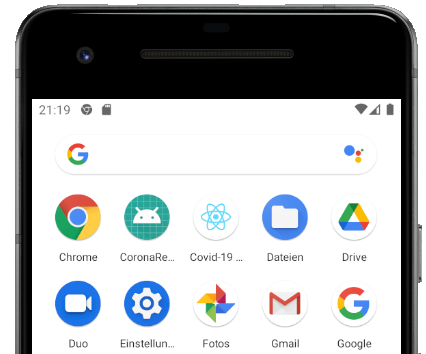
\includegraphics[width=0.5\textwidth]{figures/PWA_RN_installed.png}}
\subfigure[PWA im Startbildschirm auf einem iOS Gerät]{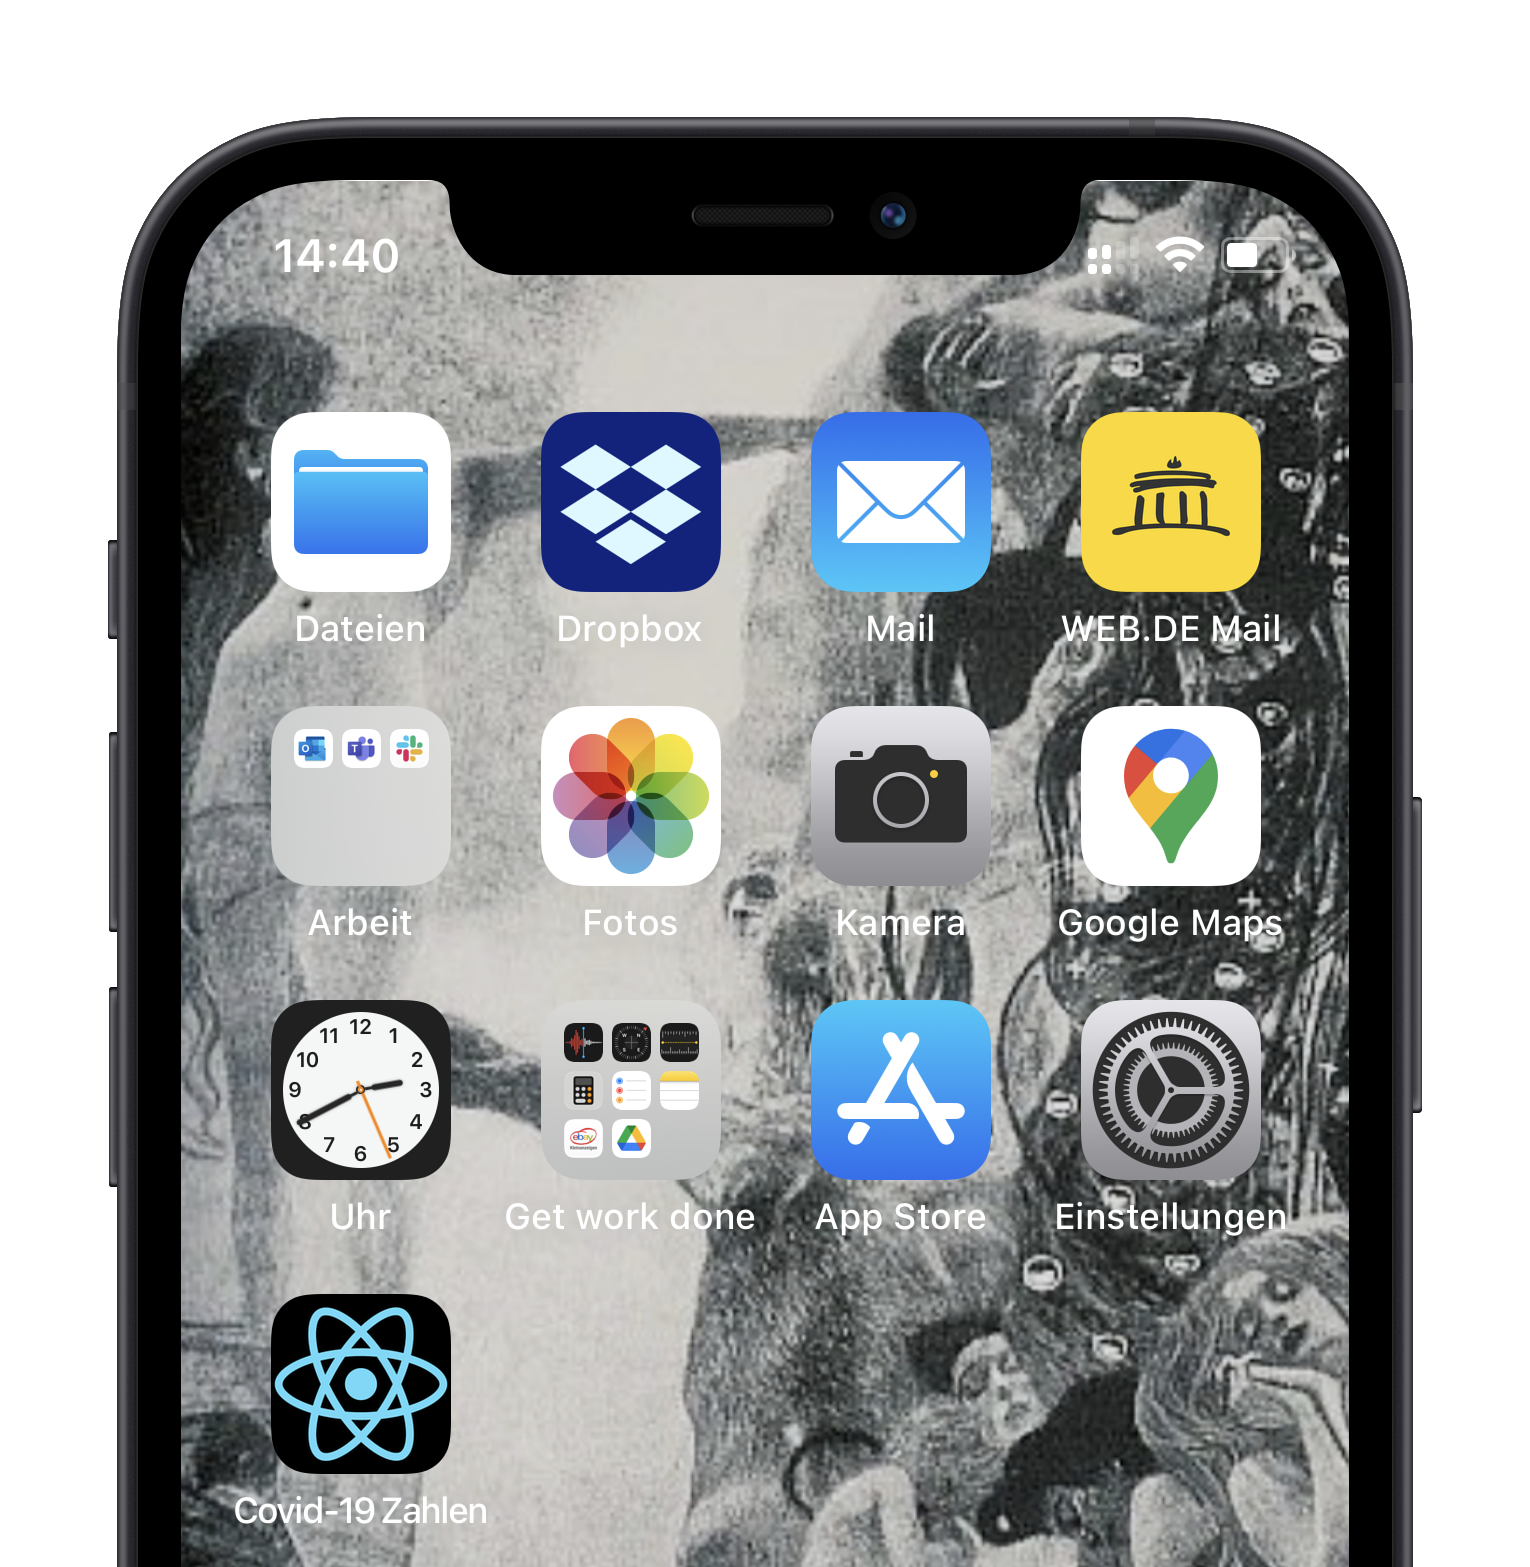
\includegraphics[width=0.5\textwidth]{figures/PWA_installed.png}}
\caption{Darstellung der installieren Apps}
\label{fig:pwa_rn_installed}
\end{figure}

Auf dem Startbildschirm sind die Anwendungen in iOS optisch nicht voneinander unterscheidbar.
Mit dem genutzten Emulator wird demgegenüber in der Chrome Version 83 durch ein kleines Browser-Symbol auf dem App-Icon deutlich, dass es sich hierbei um eine Webanwendung handelt.
In aktuelleren Browserversionen wie Chrome 91 entfällt auch dieses Symbol, wodurch \acp{pwa} auf Android Geräten ebenfalls wie Native Apps aussehen.
Mittlerweile können auch Begrüßungsbildschirme\footnote{Wenn eine App gestartet wird, zeigt sie einige Sekunden eine Art Ladebildschirm an, bis sie bereit ist.
Dabei wird meist das Logo der App und eine Hintergrundfarbe angezeigt.} für \acp{pwa} implementiert werden, wenn die Attribute \textit{name}, \textit{background\_color} und \textit{icons} im App Manifest vorhanden sind \cite{LePage.2021}.

Ein Vorteil von \acp{pwa} ist dennoch, dass sie grundsätzlich nicht installiert werden müssen.
Alle Funktionalitäten wie Standortzugriff oder Push Benachrichtigungen können aus dem Web heraus geschehen.
Native Apps hingegen können erst genutzt werden, wenn sie installiert sind.
Somit können Nutzer, deren Speicherplatz nicht für die Anwendung ausreicht, diese nicht benutzen.
Die in dieser Arbeit entwickelten Apps benötigt generell wenig Speicherplatz, da die Daten vor allem vom Server abgerufen werden, aber auch hier macht sich der Unterschied bemerkbar: die React Native App verbraucht 66.02 MB und die \ac{pwa} nur circa 0.28 MB.
Das ist darauf zurückzuführen, dass die \ac{pwa} generell weniger Ressourcen verbraucht, da es sich um gängige Webtechnologien handelt.
Gerade bei der React Native App gibt es viele Hintergrundprozesse, die Speicherplatz benötigen, um die Kommunikation zwischen Main Thread und JavaScript Thread zu ermöglichen.
Aber auch beim Vergleich zwischen klassischen, nativen Anwendungen und \ac{pwa} ist der Unterschied ähnlich: Android Apps benötigen durchschnittlich 25 MB Speicherplatz \cite{Bijlani.2021}.

Im Allgemeinen verbraucht die Installation einer \ac{pwa} außerdem weniger Datenvolumen als die einer Native App.
Ein Beispiel dafür ist die Twitter Lite \ac{pwa}, welche im Gegensatz zu den 23.5 MB der Twitter Android App lediglich 0.6 MB verbraucht \cite{Google.o.J.}.
Dies ist aber kritisch zu betrachten, da \acp{pwa} Inhalte in neuen Routen erst laden, wenn diese aufgerufen wird und somit auf langer Sicht ebenfalls so viel Datenvolumen verbrauchen können wie Native Apps.

Ferner ist es möglich, \acp{pwa} im Google Play Store zu veröffentlichen, wodurch sie einerseits durch das Web, anderseits durch den Store für Nutzer zur Verfügung stehen.
Somit können Entwickler zur Verbesserung der Auffindbarkeit der Anwendung sowohl SEO\footnote{SEO ist kurz für Suchmaschinenoptimierung} als auch ASO\footnote{Kurz für App-Store-Optimierung} durchführen.
%Da sie dennoch unabhängig von App Stores sind und entstehen für Veröffentlichung keine zusätzlichen Kosten.
%Auch bei Einnahmen der App beispielsweise durch In-App-Käufen können keine Teilbeträge verlangt werden.
Der Apple App Store unterstützt die Veröffentlichung von \acp{pwa} aktuell nicht.
Dennoch sind \acp{pwa} generell unabhängig von App Stores, da sie über das Internet erreichbar sind.
Gerade dies kann allerdings eine Schwachstelle von \acp{pwa} darstellen, da sie trotz der Veröffentlichung über HTTPS, im Gegensatz zu Native Apps keine manuelle Verifizierung zur Veröffentlichung durchlaufen müssen.

Ein entwicklungstechnischer Vorteil von \acp{pwa} gegenüber nativen Apps ist, dass sie einfacher zu verwalten sind.
Wenn es eine neue Version der Anwendung gibt, wird das Deployment durchgeführt und jeder Nutzer erhält automatisch die aktuelle Version.
Bei nativen Applikationen steckt ein Mehraufwand dahinter, da sie signiert und verifiziert werden müssen, um dann vom Nutzer aus dem jeweiligen Store aktualisiert werden zu können.\\
Diese Art von Verwaltung bei \acp{pwa} hat für die Entwickler außerdem den Vorteil, dass die Nutzer stets die neuste Version der Anwendung besitzen.
Somit ist vor allem bei langjährigen Projekten, in denen sich eventuell Schnittstellen über die Zeit ändern, Persistenz bei der Nutzung der App garantiert und es muss keine Abwärtskompatibilität implementiert werden.
Dadurch können Entwicklungs- und Wartungskosten der Anwendung reduziert werden.

\subparagraph{Offlinebetrieb\\}
Beide Anwendungen wurden auf ihre Weise offlinefähig implementiert.
Bei der \ac{pwa} bedeutet dies, dass ein Service Worker programmiert werden muss, der durch die Cache API-Anfragen abspeichert und diese bei Offlinebetrieb nutzt.
Hierbei wurden verschiedene Caching-Verfahren betrachtet und diejenige ausgewählt, die am besten zur Anwendung passt.\\
In der React Native App wurde der \textit{AsyncStorage} implementiert.
Die Daten, die durch die Netzwerkanfrage zur Verfügung stehen, werden in dessen persistente Speicher hinterlegt und genutzt, wenn keine Internetverbindung besteht.
Sie bestehen auch weiterhin, wenn die Anwendung komplett geschlossen wird.
Sobald die Verbindung wieder hergestellt wird, werden die Daten erneut aus dem Internet geladen.\\
Der Unterschied in der Implementierung des Offlinebetriebs ist, dass bei der \ac{pwa} auf fehlschlagende Netzwerkanfragen reagiert und bei der Native App der Stand der Internetverbindung abgefragt wird.
Somit werden bei der nativen Anwendung trotz der vermeintlichen \glqq Network, falling back to cache\grqq{}-Strategie nicht mehr Ressourcenanfragen gestellt als bei der \ac{pwa}.

Die Anwendungen unterscheiden sich insofern nicht voneinander, dass beide erst nach der Installation offline verfügbar sind.
Für die \ac{pwa} bedeutet dies, dass sie zumindest einmal aufgerufen werden muss.
Denn nur wenn der Service Worker installiert und aktiviert ist, hat er die Fähigkeit, im Falle eine fehlenden Netzwerkverbindung mit zwischengespeicherten Daten zu reagieren.
Die React Native App muss ebenfalls durch das Herunterladen aus einem App Store installiert werden.
In beiden Fällen ist es außerdem möglich Vorgänge, die im Offlinebetrieb durch den Nutzer vorgenommen werden, zurückzustellen und erst auszuführen, wenn der Internetzugriff wiederhergestellt ist.
Für die \ac{pwa} bedeutet dies, dass die Background Sync \ac{api} implementiert werden muss.
%Native Anwendungen

%Ein weitere Aspekt ist, dass dem Nutzer im Offlinebetrieb bei der \ac{PWA} ähnlich wie bei Native Apps eine App Shell\footnote{•} zur Verfügung gestellt wird.
%Dies ermöglicht es, dass er zumindest eine minimale \ac{ui} nutzen und durch die Anwendung navigieren kann.
%In beiden Fällen wird auch bei Anfragen an das Netzwerk, beispielsweise für Daten aus der Datenbank, eine Internetverbindung benötigt.
%Dadurch ist der Offlinebetrieb in beiden Anwendungen gleichermaßen umgesetzt.

\subparagraph{Standortzugriff\\}
Der Standortzugriff konnte in beiden Anwendungen gleichermaßen realisiert werden.
In der \ac{pwa} wird dafür die Geolocation \ac{api} des Webs verwendet und bei der React Native App durch eine Bibliothek im Hintergrund auf die Google Location Service \ac{api} in Android und Core Location \ac{api} in iOS zugegriffen.

Ein Nachteil der \ac{pwa} bei dieser Funktionalität ist, dass durch die Geolocation \ac{api} lediglich der Zugriff auf die Koordinaten des Standorts oder das Beobachten der Position möglich ist.
Bei nativen Anwendungen gibt es in beiden Betriebssystemen inkludierte Schnittstellen (\textit{Geocoder} und \textit{CLGeocoder}), mit denen das Reverse Geocoding durchgeführt werden kann.
Dadurch entfällt bei Native Apps die Nutzung von externen Dienstleistern zur Bestimmung der Aufenthaltsort.

Außerdem ist die Geolocation \ac{api}, die in der \ac{pwa} genutzt wird, abhängig von einer aktiven Internetverbindung.
Dies ist bei Native Apps nicht der Fall, denn mobile Endgeräte können durch das verbaute GPS auf den aktuellen Standort des Nutzers zugreifen.

Zuletzt ist bei \acp{pwa} im Gegensatz zu nativen Apps die Weiterverarbeitung der Standortdaten im Sinne von beispielsweise Geofencing\footnote{Geofencing bezeichnet das Auslösen von Benachrichtigungen beim Betreten oder Verlassen von definierten Bereichen und Orten.} nicht möglich.
Ein Entwurf einer Spezifikation zur Implementierung einer solchen Funktion von 2017 ist von W3C als obsolet markiert \cite{GeofencingAPI.2017}.
% Eigentlich gibt es auch 	die watchPostion-Funktion, wieso kann die nicht für Geofencing genutzt werden?

Gerade für das Geofencing ist darüber hinaus die Genauigkeit der Koordinaten relevant.
Ein Beispiel dafür ist das Benachrichtigen des Nutzers beim Betreten unterschiedlicher Räume in einer Wohnung, ferner aber auch das Bestimmen des Standorts eines verlorengegangenen Geräts.
Für die implementierte App ist die Genauigkeit der Koordinaten nicht von Bedeutung, da lediglich die Stadt ermittelt werden soll, in welcher der Nutzer der App sich befindet.
Beim Testen wird jedoch deutlich, dass die Koordinaten, wie in Abbildung \ref{fig:comparison_geoloc}, exakt übereinstimmen.

\begin{figure}[h]
\subfigure[Standortbestimmung PWA]{
\includegraphics[width=0.49\textwidth]{figures/Geoloc_PWA.png}}
\subfigure[Standortbestimmung React Native App]{
\includegraphics[width=0.49\textwidth]{figures/Geoloc_RNA.png}}
\caption{Darstellung der bestimmten Koordinaten}
\label{fig:comparison_geoloc}
\end{figure}
%Paper FULLTEXT01.pdf
%Aus technischer Sicht außerdem interessant, dass die Geolocation API, die in der PWA genutzt wird, eine bessere Performance unter Beweis stellt als der Standortzugriff einer Android App.
%Wieso? Beweise?

\subparagraph{Kontaktzugriff\\}
Diese Funktionalität wurde mit der Contact Picker API implementiert.
Durch sie ist es möglich aus den vorhandenen Kontakten des Geräts einen Kontakt auszuwählen und auf dessen Daten, darunter auch die Adresse, zuzugreifen.\\
Mit React Native gibt es keine Probleme mit der Umsetzung.
Durch das Einbinden einer \textit{Bridge} mittels einer externen Bibliothek konnte diese Funktionalität programmiert werden.

Der Zugriff auf eine grundlegende Schnittstelle wie der Kontaktliste ist für native Anwendungen selbstverständlich.
Dabei ist sowohl das Lesen als auch die Erstellung und Modifikation von Kontakten möglich.
Die Contact Picker \ac{api} bietet hingegen aktuell nur das Lesen der Kontaktliste an.
Das geschieht in einer browsereigenen Darstellungform, die in \ref{fig:contact_picker_ui} für den Chrome Browser abgebildet ist.
Entwürfe für das Erweitern der Funktionalität dieser \ac{api} liegen aktuell nicht vor.

\begin{figure}[h]
 \centering
 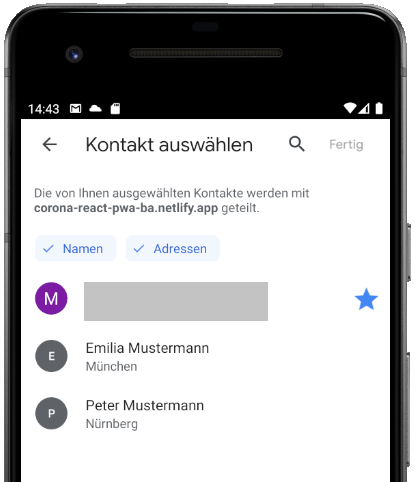
\includegraphics[width=0.6\textwidth]{figures/contact_picker_ui.png}
 \caption{Benutzeroberfläche der Contact Picker \ac{api} in Chrome}
 \label{fig:contact_picker_ui}
\end{figure}

\subparagraph{Benachrichtigungen\\}
Optisch lassen sich die Benachrichtigungen von \acp{pwa}, wie in Abbildung \ref{fig:pushnotifications_comparison} zu erkennen ist, nicht von denen von Native Apps unterscheiden.
Dies ist damit zu erklären, dass in beiden Fällen auf die betriebssystemspezifische Benachrichtigungsfunktion zugegriffen wird.
Auch im Aspekt Aktionen bieten die zwei Apps dieselben Möglichkeiten.
Bei beiden ist es möglich, Aktionen zu definieren, die von der Benachrichtigungszeile aus getätigt werden können.
Das betrifft beispielsweise das Beantworten einer Nachricht oder das Löschen einer E-Mail.

\begin{figure}[h]
 \centering
 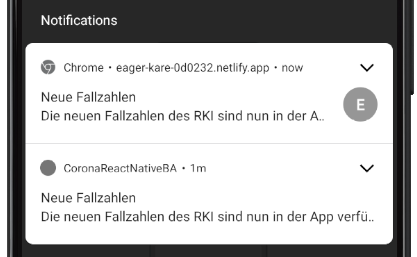
\includegraphics[width=0.6\textwidth]{figures/Push_notifications.png}
 \caption{Vergleich Benachrichtigungen PWA (oben) und React Native App (unten)}
 \label{fig:pushnotifications_comparison}
\end{figure}

Dennoch wird bei den Benachrichtigungen eine weitere Schwachstelle von \acp{pwa} deutlich.
Der Safari Browser erlaubt auf mobilen Endgeräten aktuell weder persistente noch nicht-persistente Benachrichtigungen von Webanwendungen.
Laut \textit{caniuse} implementiert der Safari Browser eine eigene Version der Push API, die jedoch nicht für Safari auf iOS verfügbar ist \cite{caniuse.com.2021}.
%Woran liegt es, dass es von Apple noch nicht unterstützt wird sich das in Zukunft ändern?

\subparagraph{Zusammenfassung\\}
Generell besitzt das Web alle Schnittstellen, um die im Kapitel \ref{ch:catalog} definierten Funktionalität umzusetzen.
Bei der Implementierung der Funktionalitäten wird dennoch deutlich, dass \acp{pwa} nicht beliebige native Schnittstellen aufrufen können, sondern lediglich Webschnittstellen nutzen.
Diese befinden sich noch im Aufbau und sind deshalb nicht umfassend, als experimentell markiert, nicht von jedem Browser unterstützt oder existieren nicht.
Das hat bei der Verwendung jener Schnittstellen zufolge, dass sich im Laufe der Zeit Schnittstellen verändern, ersetzt oder sogar entfernt werden.
Deshalb sollten diese mit Vorsicht genutzt werden.
Beispielsweise ist das App Manifest aktuell vom \textit{W3C} als experimentell gekennzeichnet und die Contact Picker \ac{api} noch ein inoffizieller Entwurf \cite{MDNcontributors.d}\cite{Beverloo.2021}.

\section{Kompatibilität mit verschiedenen Betriebssystemen} 
Durch das Testen der Apps auf jeweils einem iOS und einem Android Smartphone soll nun die Kompatibilität der beiden Anwendungen überprüft werden.
Hierfür wird ein Apple IPhone 12 mit iOS 14 und ein Huwaei P10 Lite mit Android 10 verwendet.
Die Native App wird mit einem Google Pixel 4 Emulator mit Android 11 getestet.

\subparagraph{Progressive Web App\\}
Die \ac{pwa} ist unter dem Link \url{https://corona-react-pwa-ba.netlify.app/} erreichbar.
Hierdurch kann sie mit jedem Browser eines internetfähigen Geräts erreicht werden, wodurch sie größtenteils betriebssystemunabhängig sind.
Falls ein Browser dennoch gewisse Funktionalitäten der \ac{pwa} nicht unterstützt, wird durch den Ansatz des Progressive Enhancements sichergestellt, dass die Seite zumindest die aktuellen Corona-Daten darstellt und diese nach dem Namen des Landkreises filtern kann.

In der Tabelle \ref{fig:compability_android} sind die Ergebnisse des Testens aufgelistet.
In Klammern dahinter steht zusätzlich jeweils die Browserversion, ab dem laut \textit{MDN Web Docs} diese Funktionalität unterstützt wird.
Bei der Verwendung eines Android Geräts können die meisten Funktionen genutzt werden, lediglich der Kontaktzugriff entfällt auf dem Firefox Webbrowser.
Für die Installation mit Opera gibt es von \textit{MDN Web Docs} keine Angaben über die Browserversion.
Diese Funktionalität konnte jedoch beim Testen mit der Opera Version 64 nachgewiesen werden.
Über die Nutzung der \ac{pwa} auf einem Android Gerät mit dem Safari Browser konnten keine Daten erhoben werden, da die Safari App im Google Play Store nicht zu Verfügung steht.

\begin{table}[h]
\centering
\caption{Kompatibilität der Progressive Web App mit verschiedenen Browsern auf einem Android Gerät}
\begin{tabular}[h]{|c||c|c|c|c|}
\hline
\textbf{Funktionalität} & \multicolumn{4}{|c|}{\textbf{Browser auf Android Gerät}} \\
\hline
 & Chrome & Firefox & Opera & Safari \\
\hline
Installation & ja (39) & ja (53) & ja (\kA) & - \\
\hline
Offlinebetrieb & ja (40) & ja (39) & ja (27) & - \\
\hline
Standortzugriff & ja (18) & ja (4) & ja (11) & - \\
\hline
Kontaktzugriff & ja (80) & nein & ja (57) & - \\
\hline
Benachrichtigung & ja (42) & ja (44) & ja (37) & - \\
\hline
\end{tabular}
\label{fig:compability_android}
\end{table}

Die Tabelle \ref{fig:compability_ios} zeigt die Ergebnisse der Kompatibilität bei Nutzung eines iOS Geräts.
Hierbei wird deutlich, dass die \ac{pwa}, wenn sie im Chrome, Opera oder Firefox Webbrowser aufgerufen wird, nicht die Funktionalität der Installation unterstützt.
Das ist damit zu begründen, dass iOS diese Browser mit WebKit rendert, statt mit den eigenen HTML-Renderern (\zB Blink für Chrome).
%Denn jede iOS App muss laut Punkt 2.5.6 der Apple App Store Review Guidelines als Engine WebKit nutzen \cite{Apple.07.06.2021}.
%einfach nicht supported https://support.google.com/chrome/answer/9658361?hl=en&co=GENIE.Platform%3DiOS
Ferner fehlt die Unterstützung des Kontaktzugriffs und Push Benachrichtigungen.
Ersteres ist seit iOS Version 14.15 und Safari 14.1 auch bei iOS Gerät als experimentelle Funktion verfügbar, jedoch ist das nur auf die Kontaktdaten \textit{name}, \textit{email} und \textit{tel} (Telefonnummer) beschränkt \cite{Firtman.2021}.
Dennoch zeigt dies, dass sich Apple einer Implementierung moderner Browserschnittstellen für den Safari Browser annähert.
Über eine Umsetzung von Push Benachrichtigungen auf mobilen Endgeräten gibt es aktuell keine Auskünfte \cite{Firtman.2021}.

\begin{table}[h]
\centering
\caption{Kompatibilität der Progressive Web App mit verschiedenen Browsern auf einem iOS Gerät}
\begin{tabular}[h]{|c||c|c|c|c|}
\hline
\textbf{Funktionalität} & \multicolumn{4}{|c|}{\textbf{Browser auf iOS Gerät}} \\
\hline
 & Chrome & Firefox & Opera & Safari \\
\hline
Installation & nein & nein & nein & ja (11.3) \\
\hline
Offlinebetrieb & ja (40) & ja (44) & ja (27) & ja (11.3) \\
\hline
Standortzugriff & ja (18) & ja (4) & ja (11) & ja (3) \\
\hline
Kontaktzugriff & nein & nein & nein & teilweise (14.7) \\
\hline
Benachrichtigung & nein & nein & nein & nein \\
\hline
\end{tabular}
\label{fig:compability_ios}
\end{table}

Neben den teilweise fehlenden Funktionalitäten in bestimmen Browsern und Browserversionen ist weiteres Problem von \acp{pwa}, dass einige der verwendeten Schnittstellen als experimentell gekennzeichnet sind.
Das hat bei deren Verwendung jener Schnittstellen zufolge, dass sich im Laufe der Zeit Schnittstellen verändern oder sogar ersetzt werden.
Diese Unsicherheit kann für einige Projekte ein ausschlaggebender Faktor gegen die Implementierung einer \ac{pwa} sein.
Aktuell betrifft das \acp{api} und Technologien wie das App Manifest, die Push \ac{api} und die Funktionen der Contact Picker \ac{api} \cite{MDNcontributors.d,MDNcontributors.2021,MDNcontributors.22.06.2021}.

\subparagraph{React Native\\}
Die React Native Android App kann nach dem Ausführen des Befehls \glqq npx react-native start\grqq{} und \glqq npx react-native run-android\grqq{} auf einem Emulator oder einem angeschlossenen Android Gerät genutzt werden.
Für die Nutzung auf einem iOS Gerät muss der korrespondieren Befehl \glqq npx react-native run-ios\grqq{} auf einem Mac-PC durchgeführt werden.
Dadurch, dass bei der Entwicklung der Anwendung kein Mac-PC zur Verfügung stand, konnte nicht zeitgleich geprüft werden, ob die React Native Anwendung alle Funktionalitäten auch in iOS unterstützt.
Es wird dennoch davon ausgegangen, dass alle geforderten Funktionen wie bei der Android App funktionieren, weil alle verwendeten Bibliotheken als kompatibel mit Android und iOS gekennzeichnet sind.%Quelle?

%Generell gilt jedoch, dass native Anwendungen nur auf dem Betriebssystem installiert werden können, für das sie programmiert wurden.
%Das heißt, dass eine Native App beim Faktor Kompatibilität mit verschiedenen Betriebssystemen nicht vergleichbar ist mit einer \ac{pwa}.

\subparagraph{Zusammenfassung\\}
Die Unterstützung von \acp{pwa} auf Apple Geräten hat sich, seit iOS 11.3 verbessert, da durch diese Version Schnittstellen wie der Service Worker, das App Manifest oder Cache \ac{api} verfügbar sind.
Allerdings ist es, wie bereits im Kapitel \ref{ch:implementation} beschrieben, aktuell nicht möglich, Push Benachrichtigungen auf einem iOS Smartphone zu erhalten.
Das ist ein großer Nachteil von \acp{pwa}, da 26,34 Prozent des Marktanteils somit nicht bedient werden können \cite{ODea.2021}.
Vor allem die fehlende Unterstützung von Push Benachrichtigungen ist gravierend, da somit ein ausschlaggebender Faktor zur laufenden Interaktion mit den Nutzern verloren geht.
Von Apple gibt es keine Rückmeldung, ob und wann die Funktion unterstützt werden soll.\\%quelle
Die Schnittstelle für den Kontaktzugriff wurde mit der aktuellen iOS Version 14.7 veröffentlicht und ist nach der Entfernung der Experimentell-Markierung künftig vollständig verfügbar \cite{Firtman.2021}.

Von der Auswahl der verschiedenen Betriebssysteme, auf denen eine \ac{pwa} aufgerufen werden kann, hat eine \ac{pwa} mehr Reichweite.
Da die Kompatibilität jedoch lückenhaft ist, kann dies nicht als Vorteil der \ac{pwa} gesehen werden.
Vor allem die fehlende Unterstützung von iOS Geräten spricht gegen deren Etablierung.
Eine React Native App verspricht mehr Kompatibilität als eine Native App, jedoch konnte auch dies nicht bestätigt werden, da die iOS App in diesem Falle bereits beim Aufsetzen der Entwicklungsumgebung gescheitert ist.
Bei einer Ausstattung mit einem Mac-Computer wäre dies weniger problematisch, denn dort ist eine zeitgleiche Entwicklung für iOS und Android möglich.
Dies trifft ebenso für die Nutzung des Expo Frameworks zu, da dadurch auch auf einem Windows Computer eine auf beiden Betriebssystemen lauffähige App entwickelt werden kann.
Native Apps selbst sind nach wie vor betriebssystemabhängig, wodurch sich die Kompatibilität mit verschiedenen Betriebssystemen erübrigt.

Zusammenfassend bedeutet dies dennoch, dass \acp{pwa} in Bezug auf Kompatibilität mit verschiedenen Betriebssystemen Native Apps voraus sind, da sie generell auf beiden betrachteten Betriebssystemen lauffähig sind.
Die Unterstützung einzelner Funktionalitäten ist wiederum eine Schwachstelle von \acp{pwa}, da manche nicht auf iOS Geräten existieren.
Plattformunabhängige Apps hingegen bieten -- wenn eine geeignete Entwicklungsumgebung zur Verfügung steht -- für die geforderten Funktionalitäten am meisten Kompatibilität mit verschiedenen Betriebssystemen.

\section{Entwicklungsaufwand}
Zur Bestimmung des Entwicklungsaufwand wurde einerseits die Dauer der Recherche gemessen und andererseits die reine Implementierungsdauer.
Ersteres umfasst dabei die Einarbeitung in Technologien und das Studieren der Spezifikationen, die für die Funktionalitäten benötigt werden.
Die Anwendungen wurden mit einem soliden Grundwissen in HTML, CSS und JavaScript entwickelt.
Tiefgehende Kenntnisse der Bibliothek und des Frameworks waren vor der Programmierung der Apps nicht vorhanden.
In der Tabelle \ref{fig:outlay_comparison} ist die Auflistung der Aufwände dargestellt.

\begin{table}[h]
\centering
\caption{Entwicklungsaufwand der beiden Anwendungen}
\begin{tabular}[h]{|p{3cm}||c|c|c|c|}
\hline
\textbf{Funktionalitäten} & \multicolumn{2}{|c|}{\textbf{Recherche}} &\multicolumn{2}{c|}{\textbf{Implementierung}} \\
\hline
 & PWA & Native App & PWA & Native App \\
\hline
\makecell{Einrichten der\\Entwicklungs-\\umgebung} & 60 min & 240 min & 25 min & 60 min \\
\hline
Installation & 30 min & 60 min & 30 min & 15 min \\
\hline
Offlinebetrieb & 100 min & 40 min & 45 min & 30 min \\
\hline
Standortzugriff & 30 min & 45 min & 15 min & 30 min \\
\hline
Kontaktzugriff & 60 min & 45 min & 45 min & 30 min \\
\hline
Benachrichtigung & 300 min & 250 min & 120 min & 200 min \\
\hline
\hline
Gesamt & 580 min & 680 min & 280 min & 395 min \\
\hline
\end{tabular}
\label{fig:outlay_comparison}
\end{table}

Beim Einrichten der Entwicklungsumgebung konnten in beiden Fällen Toolchains zur Beschleunigung des Prozesses genutzt werden.
Dennoch hat dies bei React Native mehr Zeit beansprucht als bei dem Aufsetzen der \ac{pwa}, weil neben der Installation der CLI weitere Vorkehrungen zur Einrichtung der Umgebungsentwicklung getätigt werden mussten.
Das betrifft beispielsweise das Konfigurieren von Android Studio oder das Aufsetzen eines \ac{avd}.
Bei der \ac{pwa} musste lediglich der Befehl \glqq npx create-react-app corona-react-pwa-ba\grqq{}\footnote{Letzteres ist der Name der Anwendung und kann frei gewählt werden} ausgeführt werden und ein vollständiges Setup zum Entwickeln einer Single Page Application ist erstellt.
Diese konnte dann sofort mit Webpack auf einem Webserver gestartet und weiterentwickelt werden.\\
Die Ermöglichung der Installation hat bei \acp{pwa} circa doppelt so lange benötigt, weil konkrete Implementierungen vorgenommen werden mussten, um dies bei der \ac{pwa} zu ermöglichen.
Beispielsweise musste das App Manifest erstellt und Icons zur Verfügung gestellt werden.
Native Apps sind generell installierbar, sie müssen lediglich zur Veröffentlichung in einem App Store signiert werden.\\
Das Ermöglichen des Offlinebetriebs hat bei der \ac{pwa} mehr Zeit beansprucht, da hier die verschiedenen Arten des Cachings der Daten betrachtet und ausgewählt werden mussten.
Für die Umsetzung in der Native App wurde der gängige \textit{AsyncStorage} in Kombination mit der React Native Bibliothek \textit{NetInfo} gewählt.\\
Das Ermöglichen des Standortabfrage hat in beiden Anwendungen ungefähr gleich viel Zeit in Anspruch genommen.\\
Die Recherche für die Implementierung des Kontaktzugriffs benötigte in der \ac{pwa} länger, da diese Funktion erst seit Chrome 80 auf Android zu Verfügung steht und somit wenig Literatur vorhanden ist \cite{Beverloo.2021}.
Auch die Programmierung selbst ist aufwendiger, da der Kontaktzugriff nur mit dem Emulator über \ac{https} und nicht mit \textit{localhost} möglich ist, weshalb die \ac{pwa} stets deployt werden musste.\\
Die Benachrichtigungen sind bei React Native mit mehr Aufwand verbunden, da die Kompatibilität auf beiden betrachteten Betriebssystemen gewährleistet werden muss.
Jedoch sind die Zeiten auch hier mit Vorsicht zu betrachten, da die \ac{pwa} auf iOS generell keine Benachrichtigungsfunktion zur Verfügung stellen kann und somit möglicherweise nötige Polyfills beim Entwicklungsaufwand entfallen.\\
Der Gesamtaufwand für die Recherche und Implementierung der \ac{pwa} beträgt somit circa 16 Stunden (850 min) und fast 18 Stunden (1075 min) für die React Native App. 

Insgesamt wird deutlich, dass für die Einfindung und Implementierung der React Native App im Gegensatz zur \ac{pwa} mehr Zeit beansprucht wurde, obwohl Teile des Codes wiederverwendet werden konnten.
Besonders ausschlaggebend war dabei die Einarbeitung in die Technologien zur plattformunabhängigen Implementierung.
Denn zur Entwicklung mit React Native muss einerseits React Native verstanden und anderseits Kenntnisse in nativer Programmierung aufgebaut werden.
Dies betrifft beispielsweise den Aufbau nativer Anwendungen und die betriebssystemspezifischen Programmiersprachen.\\
Hierbei muss außerdem beachtet werden, dass in dieser Arbeit aufgrund der Tatsache, dass kein Mac-Computer zur Entwicklung der Native App für iOS vorhanden war.
Das wirkt sich insofern auf den Entwicklungsaufwand aus, dass theoretisch für die Implementierung mehr Zeit in Anspruch genommen werden muss, weil eventuell auftretende Schwierigkeiten behoben werden müssen.
Zum Beispiel ist die Einrichtung von Push Benachrichtigungen für iOS mit \textit{Firebase} ein hinzukommender Aufwand, da dies separat von der Android Version gemacht werden muss.
Somit steigt der tatsächliche Entwicklungsaufwand der React Native App zusätzlich.

Die Ergebnisse der Entwicklungsaufwände sind nach Meinung des Autors kritisch zu betrachten, da bei der Programmierung der \ac{pwa} deutlich weniger fremder Code verwendet wurde als für die React Native App.
Hier ist es nämlich Teil des Arbeitsablaufs, sich vor-implementierten Bibliotheken zu bedienen, da oftmals \textit{Bridges} für gängige Funktionalitäten bereits existieren.
Würden diese nicht verwendet werden, wäre der Entwickungsaufwand der React Native App deutlich höher.
Auch für die \ac{pwa} könnten Bibliotheken und Werkzeuge genutzt werden, wie etwa das bereits erwähnte Tool \glqq Workbox\grqq{} von Google.
Dennoch spricht es für die \ac{pwa}, dass keine Abhängigkeit von anderen Bibliotheken benötigt werden, sondern die Funktionalität lediglich durch moderne Schnittstellen geschieht, die das Web anbietet.
Eine Native mit Java oder Swift implementierte App besitzt ebenso weniger Abhängigkeiten als die React Native App, da sie auf die nativen Schnittstellen der Betriebssysteme zugreifen.
Diese Abhängigkeit ist also nur eine Besonderheit von React Native Apps.

Außerdem ist an dieser Stelle anzumerken, dass der Entwicklungsaufwand einer mit React Native entwickelten App nicht gleichzusetzen ist mit einer tatsächlich nativen App.
Diese benötigt für dasselbe Ergebnis zwei Implementierungen, eine für Android und eine für iOS.
Dadurch kann sich der Recherche- und Entwicklungsaufwand verdoppeln, zumal auch eine Einarbeitung in zwei verschiedene Programmiersprachen und Entwicklungsumgebungen stattfinden muss.

Ein großer Nachteil der Entwicklung mit React Native ist, dass aktuell nicht komplett plattformunabhängig programmiert werden kann.
So ist ein Mac-Computer die Voraussetzung zur Implementierung von nativen iOS Komponenten in einer React Native Anwendungen.
Das betrifft auch die Ansprache von spezifischen Schnittstellen wie Touch oder Face ID, Bluetooth und selbst Batterieverbrauch von iOS Geräten. %Quelle
Theoretisch können auch externe Dienstleister diese Teile der Implementierung übernehmen, jedoch bringt das weitere Entwicklungskosten und eine höheren Managementbedarf.
Im Gegensatz dazu sind \acp{pwa} in der Entwicklung grundlegend unabhängig, da es sich dabei um normale Webanwendungen handelt, welche keine spezifische Entwicklungsumgebung benötigen.

Ferner muss betont werden, dass es sich bei React Native App trotz der Programmierung großer Teile in JavaScript im Endeffekt um zwei Technologien handelt, die der Entwickler beherrschen muss.
Einerseits JavaScript für das Implementieren einer Anwendung mit React, andererseits das Wissen über native Entwicklung, Schnittstellen und betriebssystemabhängige Programmiersprachen, um gegebenenfalls plattformspezifischen Code zu ergänzen.
Das wirkt sich insofern auf den Entwicklungsaufwand aus, dass JavaScript-Entwickler, die keine Erfahrungen mit nativer App-Entwicklung haben, mehr Zeit für die Einarbeitung in die Thematik benötigen.

\begin{figure}
\subfigure[React App Texteingabe Implementierung]{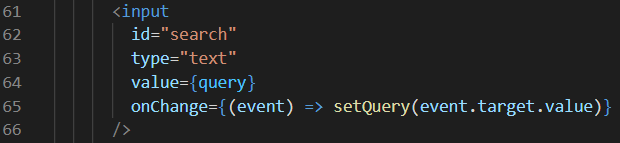
\includegraphics[width=0.49\textwidth]{figures/Input_R.png}}
\subfigure[React Native Texteingabe Implementierung]{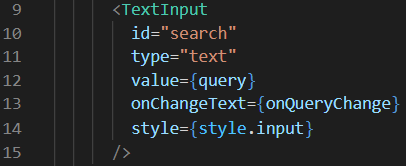
\includegraphics[width=0.49\textwidth]{figures/Input_RN.png}}
\caption{Vergleich Implementierung React PWA und React Native App}
\label{fig:textinputComparison}
\end{figure}

Ein besonderer Vorteil dieser Konstellation von Technologien ist jedoch, dass Teile der Logik und Aufteilung der Komponenten aus der React Web App in die React Native App übernommen werden können und somit Zeit gespart wird.
Ein Beispiel dafür ist in der Abbildung \ref{fig:textinputComparison} verdeutlicht.
Hieran wird sichtbar, dass in vielen Fällen die Syntax nur abgeändert werden muss, um die React Version der Implementierung in React Native zu übertragen.
Das ist vor allem dann eine Option, wenn im Laufe des Projekts klar wird, dass die Funktionalitäten, die \acp{pwa} aktuell anbieten, nicht ausreichen.
Diese Art von flexibler Entwicklung bieten native Anwendungen grundsätzlich nicht.

\section{Bewertung der Technologien anhand des Kriterienkatalogs}
In der Tabelle \ref{fig:discussion_impl} soll nun auf Grundlage der dargestellten Argumente die Erfüllung der einzelnen Kriterien in Form von Punkten bewertet werden.
Diese beruht auf den in Kapitel \ref{ch:catalog} festgelegten Definitionen der Erfüllung.\\
Auf eine Gewichtung der Kriterien wurde durch den Anwendungsfall bewusst verzichtet.
Der Grund hierfür ist, wie bereits erwähnt, dass sowohl die Funktionalität als auch die Kompatibilität und der Entwicklungsaufwand für den Anwendungsfall von gleicher Bedeutung sind.


\begin{table}[ht]
\centering
\caption{Nutzwertanalyse der beiden implementierten Anwendungen}
\begin{tabular}{|ll|c|c|}
\hline
\multicolumn{1}{|c}{\textbf{Kriterium}}               & \multicolumn{1}{c|}{} & \textbf{PWA} & \textbf{Native App} \\ \hline
\multicolumn{1}{|l|}{\multirow{5}{*}{Funktionalität}} & Installation          & 1            & 0                   \\ \cline{2-4} 
\multicolumn{1}{|l|}{}                                & Offlinebetrieb        & 1            & 1                   \\ \cline{2-4} 
\multicolumn{1}{|l|}{}                                & Standortzugriff       & 1            & 2                   \\ \cline{2-4} 
\multicolumn{1}{|l|}{}                                & Kontaktzugriff        & 1            & 2                   \\ \cline{2-4} 
\multicolumn{1}{|l|}{}                                & Benachrichtigungen    & 2            & 2                   \\ \hline
\multicolumn{2}{|l|}{Kompatibilität mit vers. Betriebssystemen}               & 2            & 3 (1)               \\ \hline
\multicolumn{2}{|l|}{Entwicklungsaufwand}                                     & 2            & 0                   \\ \hline
\multicolumn{2}{|l|}{\textbf{Summe}}                                          & \textbf{10}  & \textbf{10 (8)}     \\ \hline
\end{tabular}
\label{fig:discussion_impl}
\end{table}

Beim Kriterium der Funktionalität kann die \ac{pwa} mit der Native App mithalten, jedoch wird deutlich, dass die Native App mehr kann.
Lediglich bei der Installation ist die \ac{pwa} durch ihre erhöhte Zugänglichkeit im Vorteil.\\
Die Kompatibilität mit verschiedenen Betriebssystemen ist bei der \ac{pwa} mit 2 Punkten versehen, da sie \ac{pwa} kompatibel mit mehreren Betriebssystemen ist, aber abhängig von dem verwendeten Browser.
Eine React Native App hingegen ist generell für mehreren Betriebssystemen verfügbar und unabhängig vom Browser.
Dennoch steht in Klammern dahinter eine geringere Punktzahl, die eine normale, native App erhalten würde, denn diese unterscheidet sich stark implementierten React Native App, da sie nur auf einem Betrieb\\
Das Kriterium des Entwicklungsaufwands erfüllt die \ac{pwa} wiederum besser, weil sowohl die Recherche- als auch die Implementierungszeit geringer war als bei der React Native App.\\
Das Ergebnis zeigt, dass beide Technologien für diesen Anwendungsfall gleich viel Punkte erhalten.
Lediglich die normale, native App, würde in diesem Vergleich weniger Punkte als die \ac{pwa} erreichen und somit für eine klare Ersatz durch \acp{pwa} sprechen.

%Beim Kriterium der Funktionalität erreichen beide Apps für den definierten Anwendungsfall die maximale Punktzahl, da alle geforderten Funktionen mit beiden Technologien umgesetzt werden können.
%Die Kompatibilität mit verschiedenen Betriebssystemen war bei \acp{pwa} nicht vollkommen gegeben, da Safari, wie bereits erläutert, einige Funktionalitäten nicht unterstützt.
%Das Kriterium des Entwicklungsaufwands erfüllt die \ac{pwa} wiederum besser, weil sowohl die Recherche- als auch die Implementierungszeit geringer war als bei der React Native App.
%Deshalb erhält die \ac{pwa} in diesem Aspekt eine höhere Punktzahl.\\
%Das Ergebnis zeigt, dass in diesem Anwendungsfall die Native App durch eine \ac{pwa} ersetzt werden kann.







%Nun sollen in einer weiteren Tabelle \ref{fig:discussion_gen} die Erfüllung der Kriterien durch die zwei Technologien im Allgemeinen betrachtet werden.
%Hierbei wurde zusätzlich eine tatsächlich Native App für den Vergleich aufgenommen, denn diese unterscheidet sich insofern, dass sie nicht kompatibel mit verschiedenen Betriebssystemen ist.
%Auch der Entwicklungsaufwand ist höher, denn um dasselbe Ergebnis zu erreichen wie bei einer PWA oder React Native App, muss für jedes Betriebssystem eine eigene App mit der jeweiligen Entwicklungsumgebung entwickelt werden.
%Im Gegensatz zur vorherigen Tabelle wird deutlich, dass \acp{pwa} weniger Funktionalitäten unterstützen als React Native oder Native Apps.
%Beispielsweise betrifft das in dieser Arbeit nicht behandelte Funktionen wie das Geofencing oder die User Idle Detection\footnote{Das Erkennen, ob der Nutzer den Bildschirm aktiv betrachtet.} \cite{AppBar.2021}.
%Die anderen Kriterien sind bei der \ac{pwa} und React Native App gleichermaßen erfüllt.\\

%Her zu ausblick als hier
%Anhand des Vergleichs der beiden Nutzwertanalysen wird klar, dass \acp{pwa} nicht allgemein als Ersatz zu nativen Anwendungen gesehen werden können.
%Die Ergebnisse legen zudem zusammenfassend nahe, dass eine Entscheidung für eine der beiden Implementationen abhängig von den Anforderungen an die zu entwickelnde App getroffen werden sollte.